\documentclass[11pt]{article}
\usepackage[margin=1.5in]{geometry}
\usepackage{graphicx}
\usepackage{float}
\usepackage{parskip}
\usepackage{amsmath}
\usepackage{pgfplots}
\pgfplotsset{width=10cm, compat=1.9}

\begin{document}

\textbf{\Huge Continuity and Limits}

Athan Zhang \& Jeffrey Chen

\section{Limits}

\subsection{Definition}
A \textbf{limit} refers to the value that a function's output approaches as the input approaches a specific number. It describes the behavior of a function at a point of interest, and is the fundamental building block upon which many concepts in calculus are built. The limit of $f(x)$ as $x$ approaches $x_0$ is written using the following notation: $\lim_{x\to x_0} f(x)$. 

\subsection{One-Sided Limits}
Limits can be taken from both the \textbf{left} and \textbf{right} hand sides. This means analyzing the behavior of $f(x)$ as $x$ approaches a certain value from the left hand side alone, or from the right hand side alone. This is important as sometimes these values differ, creating results that will be explained further in the following section. 

The left hand limit of $f(x)$ as $x$ approaches $x_0$ is written as $\lim_{x\to x_0^-} f(x)$. Similarly, the right hand limit of $f(x)$ as $x$ approaches $x_0$ is written as $\lim_{x\to x_0^+} f(x)$. It is said that $\lim_{x\to x_0} f(x)$ \textbf{exists} when $\lim_{x\to x_0^-} f(x) = \lim_{x\to x_0^+} f(x)$ and \textbf{does not exist} when $\lim_{x\to x_0^-} f(x) \neq \lim_{x\to x_0^+} f(x)$.

\subsection{Limits, Infinity and Asymptotes}
The relationship between limits and \pm \infty\;can be used to determine asymptotes of a function:

The line $y=y_0$ is a \textbf{horizontal asymptote} of the function $f(x)$ if either $\lim_{x\to \infty} f(x) = y_0$ or $\lim_{x\to -\infty} f(x) = y_0$.

The line $x=x_0$ is a \textbf{vertical asymptote} of the function $f(x)$ if either $\lim_{x\to a^+} f(x) = \pm \infty$ or $\lim_{x\to a^-} f(x) = \pm \infty$.

\subsection{End Behavior}
End behavior refers to trends exhibited by a function as its input approaches $\pm\infty$. Analyzing end behavior allows us to gain a better understanding of the overall shape and trends of a function. There are generally three types of end behavior: asymptotic, bounded, and unbounded.

\subsubsection*{Asymptotic Behavior}
A function exhibits asymptotic behavior if it approaches a horizontal asymptote, as $x$ approaches $\pm\infty$. The function may get arbitrarily close to the asymptote but never actually touch it.

\begin{center}
\begin{tikzpicture}
\begin{axis}[
    axis lines=middle, width=6cm, height=6cm, ymin=-4, ymax=4, ytick={-4, -2, 2, 4}, xmin=-4, xmax=4, ytick={-4, -2, 2, 4}
]
\addplot[color=red]{e^(-x)};
\end{axis}
\end{tikzpicture}
\end{center}

\subsubsection*{Bounded Behavior}
A function whose values remain within a certain range as $x$ approaches $\pm\infty$. This means that the function's values will never increase or decrease past a certain bound as $x$ becomes extremely large or small.

\begin{center}
\begin{tikzpicture}
\begin{axis}[
    axis lines=middle, width=6cm, height=6cm, ymin=-4, ymax=4, ytick={-4, -2, 2, 4}, xmin=-4, xmax=4, ytick={-4, -2, 2, 4}
]
\addplot[color=red]{sin(deg(x))};
\end{axis}
\end{tikzpicture}
\end{center}

\subsubsection*{Unbounded Behavior}
A function that grows without bound as $x$ approaches $\pm\infty$. This means that the function's values increase or decrease indefinitely as $x$ becomes extremely large or small. Note that a vertical asymptote is not necessary for a function to exhibit unbounded behavior.

\begin{center}
\begin{tikzpicture}
\begin{axis}[
    axis lines=middle, width=6cm, height=6cm, ymin=-4, ymax=4, ytick={-4, -2, 2, 4}, xmin=-4, xmax=4, ytick={-4, -2, 2, 4}
]
\addplot[color=red]{e^(x)};
\end{axis}
\end{tikzpicture}
\end{center}

As can be seen, the main method of analyzing the end behavior of a function is to take the limit as $x$ approaches \pm \infty.

\subsection{Finding Limits}
For many basic functions and graphs, limits can be computed rather easily either through graphical methods or numerical methods. However, finding the limits of more complex functions can be tricky, and sometimes requires the use of the following methods.

% limit rules
\subsubsection*{Limit Rules}
The following rules apply when determining limits, and can be helpful when computing limits. 

\renewcommand{\arraystretch}{1.25}
\begin{table}[H]
    \centering
    \begin{tabular}{p{3cm} p{10cm}}
    Sum Rule & $\lim_{x\to x_0} (f(x)+g(x)) = \lim_{x\to x_0} f(x) + \lim_{x\to x_0} g(x)$\\ 
    Difference Rule & $\lim_{x\to x_0} (f(x)-g(x)) = \lim_{x\to x_0} f(x) - \lim_{x\to x_0} g(x)$\\ 
    Product Rule & $\lim_{x\to x_0} (f(x)\cdot g(x)) = \lim_{x\to x_0} f(x) \cdot \lim_{x\to x_0} g(x)$\\ 
    Quotient Rule & $\lim_{x\to x_0} \frac{f(x)}{g(x)} = \frac{\lim_{x\to x_0} f(x)}{\lim_{x\to x_0} g(x)}$ provided $\lim_{x\to x_0} g(x) \neq 0$\\  
    Constant Rule & $\lim_{x\to x_0} af(x) = a\lim_{x\to x_0} f(x)$\\
    N\textsuperscript{th} Root Rule & $\lim_{x\to x_0} \sqrt[n]{f(x)} = \sqrt[n]{\lim_{x\to x_0} f(x)}$\\
    \end{tabular}
\end{table}
\renewcommand{\arraystretch}{1}

Note: When using the quotient rule, it is possible to arrive at an answer of $\frac{0}{0}$. Sometimes, this problem may be resolved through algebraic manipulation of the original function. In other cases, the analysis of the limit requires more tools, which will be introduced later in this course.

\subsubsection*{Squeeze Theorem}

Let's assume we're trying to find the limit of a function $f(x)$ given at a certain point. Let's also assume that for every value $x$, $h(x)$ is less than $f(x)$ and $g(x)$ is greater than $f(x)$ such as the following holds true.

\begin{align*}
    h(x) \leq f(x) \leq g(x)\;\forall\; x
\end{align*}

Then, if the lower and upper functions have equal limits at $x = c$ approach the same value $L$

\begin{align*}
    \lim_{x \to c} h(x) = \lim_{x \to c} g(x) = L
\end{align*}

We can squeeze the two functions and calculate that the limit at $f(c)$ is also $L$.

\begin{align*}
    \lim_{x \to c}f(x) = L
\end{align*}


\section{Continuity}

\subsection{Definition}

A function is called \textbf{continuous} when it has no abrupt interruptions in its behavior. Simply put, a continuous function can be drawn with a single, unbroken curve. 

\subsubsection*{Three-Step Test For Continuity}
More rigorously speaking, there are 3 requirements for a function $f(x)$ to be continuous at any given point $x_0$: 
\begin{itemize}
  \item $\lim_{x\to x_0} f(x)$ must exist.
  \item $f(x)$ must be defined at $x_0$.
  \item $\lim_{x\to x_0} f(x)$ must equal $f(x_0)$.
\end{itemize}

Sometimes, a function may be continuous except for one or more specific points. These points are referred to as \textbf{discontinuities}.

\subsection{Types of Discontinuities}
There are generally 4 types of discontinuities: jump discontinuities, infinite discontinuities, hole discontinuities, and endpoint discontinuities. 

\subsubsection*{Jump Discontinuities}
A jump discontinuity is defined as a point on a function where the limits from the right and left hand side are not equal. This occurs most of the time with piecewise functions.

\begin{center}
\begin{tikzpicture}
\begin{axis}[
    axis lines=middle, width=6cm, height=6cm
]
\pgfplotsset{hole/.style={color=red,fill=white,only marks,mark=*}}
\pgfplotsset{dot/.style={color=red,fill=red,only marks,mark=*}}
\addplot[domain=-4:1, color=red]{x};
\addplot[domain=1:4, color=red]{x+1};
\addplot[hole] coordinates{(1,1)};
\addplot[dot] coordinates{(1,2)};
\end{axis}
\end{tikzpicture}
\end{center}

\subsubsection*{Infinite Discontinuities}
An infinite discontinuity is defined as a point on a function where the limits from the right and left hand side approach $\pm\infty$. This occurs most of the time when dividing by $0$.

\begin{center}
\begin{tikzpicture}
\begin{axis}%
    [ 
        xmin=-4,
        xmax=4,
        axis x line=middle,
        ytick={-4, -2, 2, 4},
        ymin=-4,
        ymax=4,
        axis y line=middle,
        samples=100,
        domain=-10:10,
        restrict y to domain=-30:30,
        width=6cm, height=6cm
    ]
    \addplot[thick,samples=400, color=red] (x,{1/x});
\end{axis} 
\end{tikzpicture}
\end{center}

\subsubsection*{Hole Discontinuities}
A hole discontinuity is defined as a point on a function where the limit exists, but the function itself is not defined, or does not equal the limit. These discontinuities are referred to as "removable" due to the fact that they can often be removed from the function with a bit of algebraic manipulation.

\begin{center}
\begin{tikzpicture}
\begin{axis}[
    axis lines=middle, width=6cm, height=6cm
]
\pgfplotsset{hole/.style={color=red,fill=white,only marks,mark=*}}
\addplot[domain=-4:4, color=red]{(x-1)*x/(x-1)};
\addplot[hole] coordinates{(1,1)};
\end{axis}
\end{tikzpicture}
\end{center}

\subsubsection*{Endpoint Discontinuities}
An endpoint discontinuity is defined as the endpoint of a function's domain where the limit does not exist due to the absence of either the right or left hand side of the function. 

\begin{center}
\begin{tikzpicture}
\begin{axis}[
    axis lines=middle, width=6cm, height=6cm, ymin=-4, ymax=4, ytick={-4, -2, 2, 4}, xmin=-4, xmax=4, ytick={-4, -2, 2, 4}
]
\pgfplotsset{dot/.style={color=red,fill=red,only marks,mark=*}}
\addplot[domain=0:4, color=red]{x^(0.5)};
\addplot[dot] coordinates{(0,0)};
\end{axis}
\end{tikzpicture}
\end{center}

\subsection{Intermediate Value Theorem}
The Intermediate Value Theorem states that if $f(x)$ is a continuous function whose domain contains the interval $[a, b]$, then it takes on every value within $[f(a), f(b)]$ at some point on the interval. This theorem is mainly used to estimate the location(s) of a function's zero(s).

\section{Secants and Tangents}

\subsection{Secant Lines}

A \textbf{secant line} refers to a line connecting two points on a curve. An example of a secant line segment is shown below. 
\begin{center}
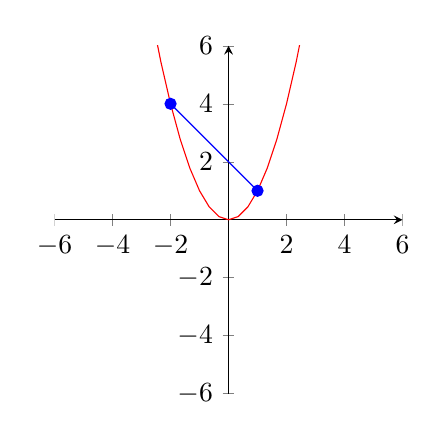
\begin{tikzpicture}
\begin{axis}[
    axis lines=middle, width=6cm, height=6cm, ymin=-6, ymax=6, ytick={-6, -4, -2, 2, 4, 6}, xmin=-6, xmax=6, xtick={-6, -4, -2, 2, 4, 6},
]
\pgfplotsset{dot/.style={color=blue,fill=blue,only marks,mark=*}}
\addplot[domain=-4:4, color=red]{x^2};
\addplot[domain=-2:1, color=blue]{-x+2};
\addplot[dot] coordinates{(-2,4)};
\addplot[dot] coordinates{(1,1)};
\end{axis}
\end{tikzpicture}
\end{center}

\subsection{Average Rate of Change}

Secant lines are useful for determining the average rate of change of a function: 
Given a function $f(x)$, the average rate of change of $f(x)$ from point $x_0$ to point $x_1$ is equal to the \textbf{slope} of the secant line between $x_0$ and $x_1$. This can also be written as the following: 

\begin{center}
\begin{equation*}
RoC_{avg} = \frac{f(x_2)-f(x_1)}{x_2-x_1}. 
\end{equation*}
\end{center}

This has many practical and contextual uses, such as determining average velocity or acceleration over a period of time, average growth rate of a quantity, et cetera.

\subsection{Tangent Lines}

Imagine a secant line passing through points $x_0$ and $x_1$ on a function $f(x)$. Now, we will investigate what happens as these two points get closer and closer to each other. Visualize taking $x_1$ and dragging it towards $x_0$. What happens to the secant line?  


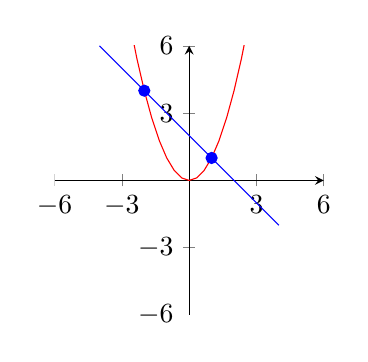
\begin{tikzpicture}
\begin{axis}[
    axis lines=middle, width=5cm, height=5cm, ymin=-6, ymax=6, ytick={-6, -3, 3, 6}, xmin=-6, xmax=6, xtick={-6, -3, 3, 6}
]
\pgfplotsset{dot/.style={color=blue,fill=blue,only marks,mark=*}}
\addplot[domain=-4:4, color=red]{x^2};
\addplot[domain=-4:4, color=blue]{-x+2};
\addplot[dot] coordinates{(-2,4)};
\addplot[dot] coordinates{(1,1)};
\end{axis}
\end{tikzpicture} \hspace{3em} 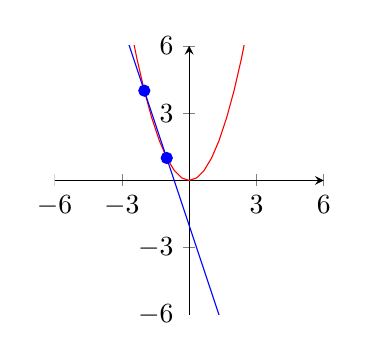
\begin{tikzpicture}
\begin{axis}[
    axis lines=middle, width=5cm, height=5cm, ymin=-6, ymax=6, ytick={-6, -3, 3, 6}, xmin=-6, xmax=6, xtick={-6, -3, 3, 6}
]
\pgfplotsset{dot/.style={color=blue,fill=blue,only marks,mark=*}}
\addplot[domain=-4:4, color=red]{x^2};
\addplot[domain=-4:4, color=blue]{-3*x-2};
\addplot[dot] coordinates{(-2,4)};
\addplot[dot] coordinates{(-1,1)};
\end{axis}
\end{tikzpicture} \hspace{3em} 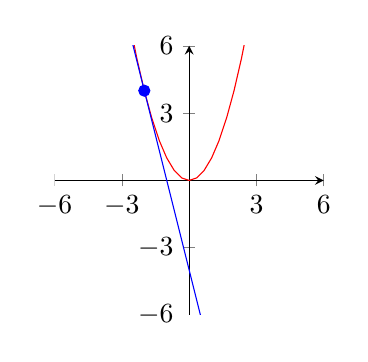
\begin{tikzpicture}
\begin{axis}[
    axis lines=middle, width=5cm, height=5cm, ymin=-6, ymax=6, ytick={-6, -3, 3, 6}, xmin=-6, xmax=6, xtick={-6, -3, 3, 6}
]
\pgfplotsset{dot/.style={color=blue,fill=blue,only marks,mark=*}}
\addplot[domain=-4:4, color=red]{x^2};
\addplot[domain=-4:4, color=blue]{-4*x-4};
\addplot[dot] coordinates{(-2,4)};
\end{axis}
\end{tikzpicture}

The line in the third figure is known as a \textbf{tangent line}, a line that touches the function at \textbf{only one} point. It can be thought of as the limit of a secant line as $x_1$ approaches $x_0$.

\subsection{Instantaneous Rate of Change}

Tangent lines are useful for determining the average rate of change of a function: 
Given a function $f(x)$, the instantaneous rate of change of $f(x)$ at the point $x_0$ is equal to the \textbf{slope} of the tangent line at $x_0$. This can also be written as the following: 

\begin{center}
\begin{equation*}
RoC_{inst} = \lim_{h \to 0} \frac{f(x_0+h)-f(x_0)}{h}. 
\end{equation*}
\end{center}

This allows us to analyze the values of a function at just a single point, a supremely useful ability, both practically and theoretically. It can be used to find instantaneous velocity, acceleration, growth rate, et cetera. 

This is also the fundamental definition of a \textbf{derivative} and is the building block of most of the concepts of calculus that will follow. Derivatives will be further explored in following units of the course.

\end{document}